\chapter{SEIR epidemic model on real contact networks and surrogates}


\section{SEIR model and dataset}
 
In the paper \cite{pung2022using}, the authors analyzed the contact data of passengers and crew members recorded on a three days cruise ship, departed from Singapore and arrived in the same port. Bluetooth bracelets recorded the duration  (in seconds) of a contact between two people on board. Each person is identified by a unique ID and the contact events are grouped by day, but there is no time ordering within a day. Each node belongs to a specifc group (passengers, crew, security, housekeep) and each contact happened in a specific area of the ship (Entartainement, Food and Beverage, Galley, Hotel).

In this task we  simulated a SEIR epidemic model on four different networks: a temporal and aggregated version of the contact network and surrogate temporal and static Erdos Renyi  (ER) models. All the networks are undirected.

In the SEIR model, the population is divided into four comparments: susceptible (\emph{S}), exposed (\emph{E}), infected (\emph{I}) and recovered (\emph{R}) individuals. The transmission of the disease and the transitions from one state to another are defined by the following probabilities:

\begin{align}\label{eq:epidemic}
    S \rightarrow E:&\quad P_{i\rightarrow j}(\Delta t_{ij}) = 1 - \exp{\frac{-\Delta t_{ij}}{r} \; \beta } \\
    E \rightarrow I:&\quad P( E \rightarrow I) = \frac{\Delta t}{\tau_E} \\
    I \rightarrow R:&\quad P( I \rightarrow R) = \frac{\Delta t}{\tau_I} \\
\end{align}


where $\Delta t_{ij}$ is the duration of a contact between  individuals $i$ and $j$ in the temporal case, while in the aggregated networks it is the weight of each edge, computed as described in the next section. The transmission probability is  $\beta$ and its value depends on the vaccinal status of $i$ and $j$ and on the use of masks; $\tau_E$ and $\tau_I$ are the recovery times from states $E$ and $I$, while $\Delta t$ is the total time spent by an individual in state $E$ or $I$. The value of $r$ scales the interaction  $\Delta t_{ij}$.





\section{Implementation}
Starting from the original data, we constructed and simulated the epidemic on the following networks:
\begin{itemize}
    \item \emph{real-temporal}: per each day of the cruise, we use the recorded list of interactions among people and their contact time to make the network. \\
    \item \emph{real-aggregated}: we considered only the unique interactions of $(i, j)$ and set the edge weight $w_{ij} = \sum_{days} \sum_{interacions} \Delta t_{ij}$ as the sum of all the contact times of the pair $(i,j)$ over the whole cruise. \\
    \item \emph{ER-temporal}: per each day, contact times are preserved, but the interacting nodes of each edge are randomly chosen among the whole set of nodes. \\
    \item \emph{ER-static}: the number of nodes and the interacting pairs are preserved, but the weights computed for \emph{real-aggregated} are randomly assigned to the edges.
\end{itemize}


The dataset is made of 2181 nodes and \num{11367586} edges for \emph{real-temporal} and \num{618278} edges for \emph{real-aggregated}.
In figure \ref{fig:distributions} we note that in the aggregated case, the strength distribution spans two orders of magnitude, while in the temporal case, both the degree and strength distributions are different per each day. 
\begin{figure}[th]
    \centering
    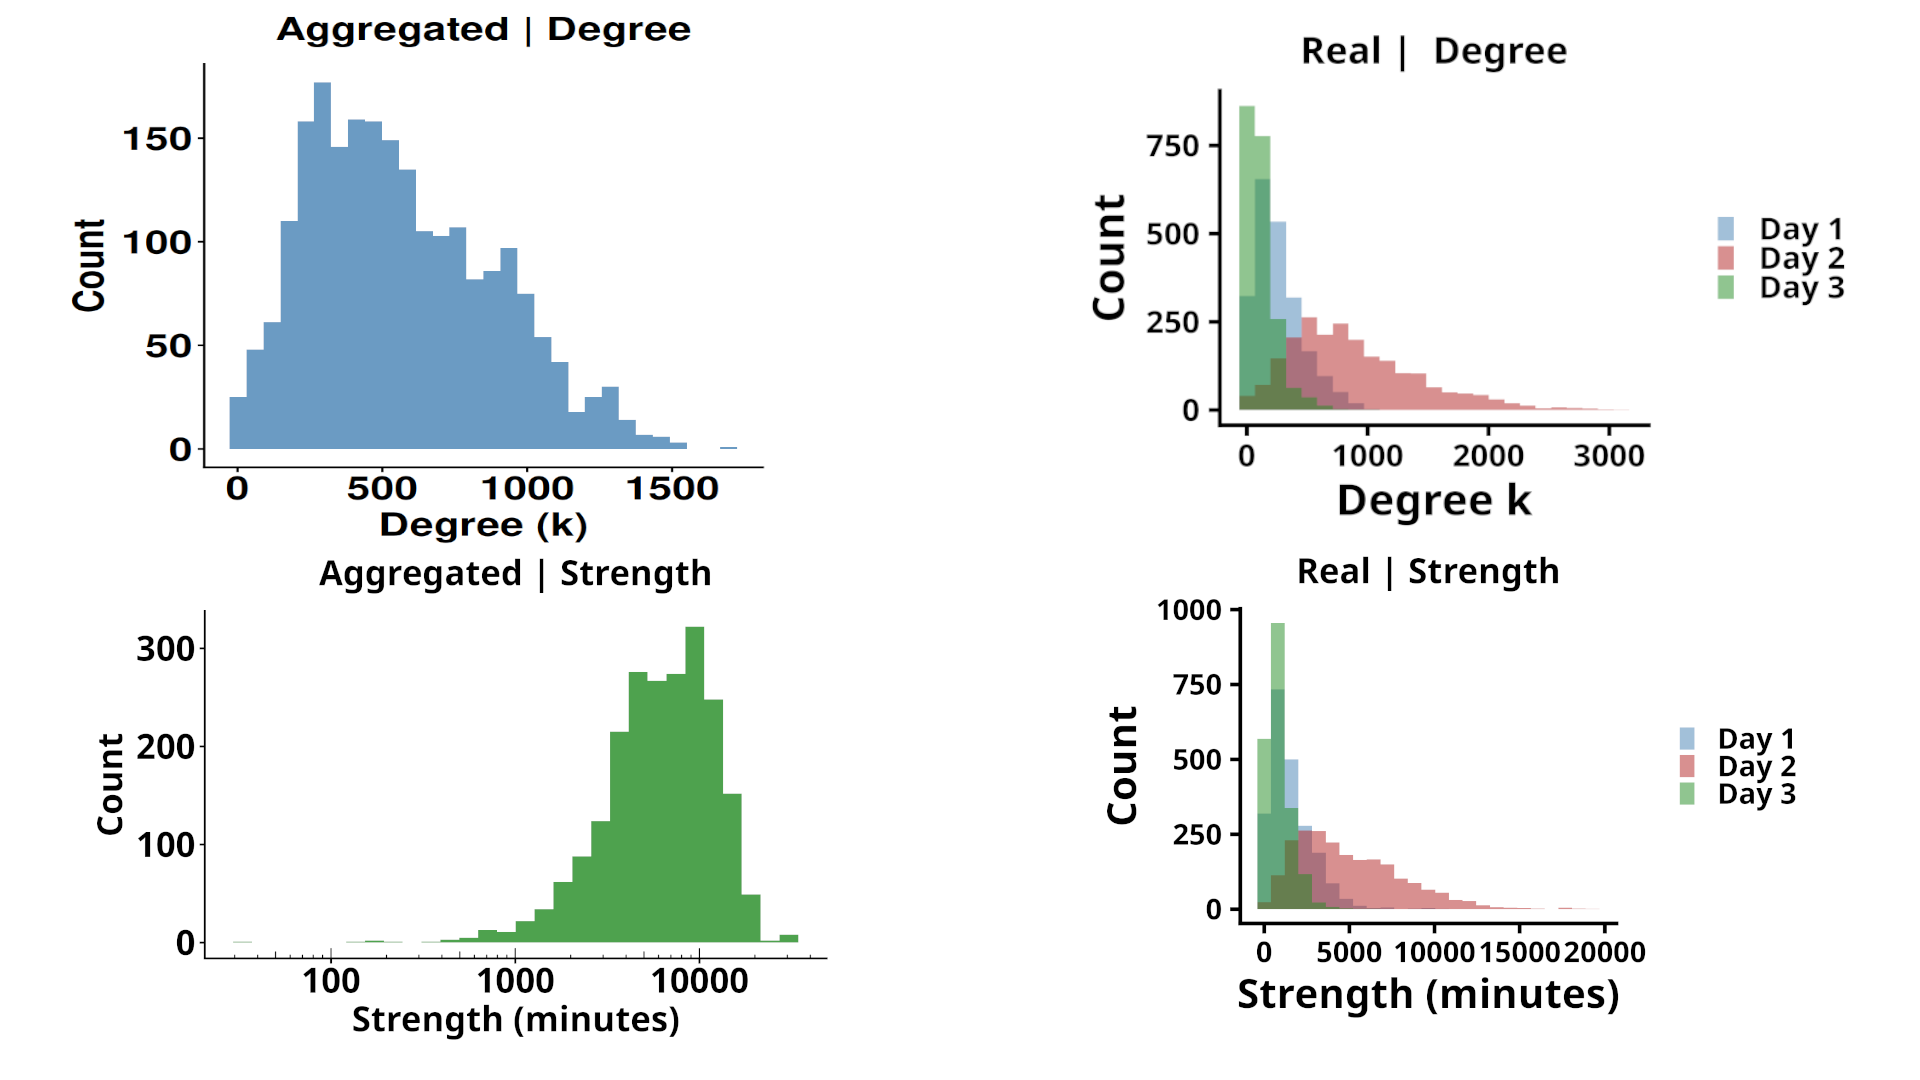
\includegraphics[width=\textwidth]{images/distributions.png}
    \caption{Degree and strength distributions of \emph{real-temporal} and \emph{real-aggregated} networks.}
    \label{fig:distributions}
\end{figure}

We simulated the epidemics in $R$ and chose the parameters values similar to the ones of the covid pandemic: $\tau_E=5 \;\text{day}^{-1}$ \cite{lauer2020incubation}, $\tau_I = 12 \;\text{day}^{-1}$, $r= 15\; \text{min}^{-1}$ \cite{alsved2023infectivity} and $\beta \in \{0.05, 0.1, 0.2, 0.25, 0.5, 1\}$ (these values have been used in \cite{pung2022using}, corresponding to contacts happening between vaccineted people or wearing a mask). We did $30$ independent runs for for each value of $\beta$, using a time step $t=1\;\text{day}$. Since the cruise lasted three days, we simulated the epidemic only for three days for every network, in order to make meaningful comprarisons. We set 1\% of the population  (sampled uniformely among all the passengers) to be infected at the starting time.

\begin{figure}[h!]
    \centering
    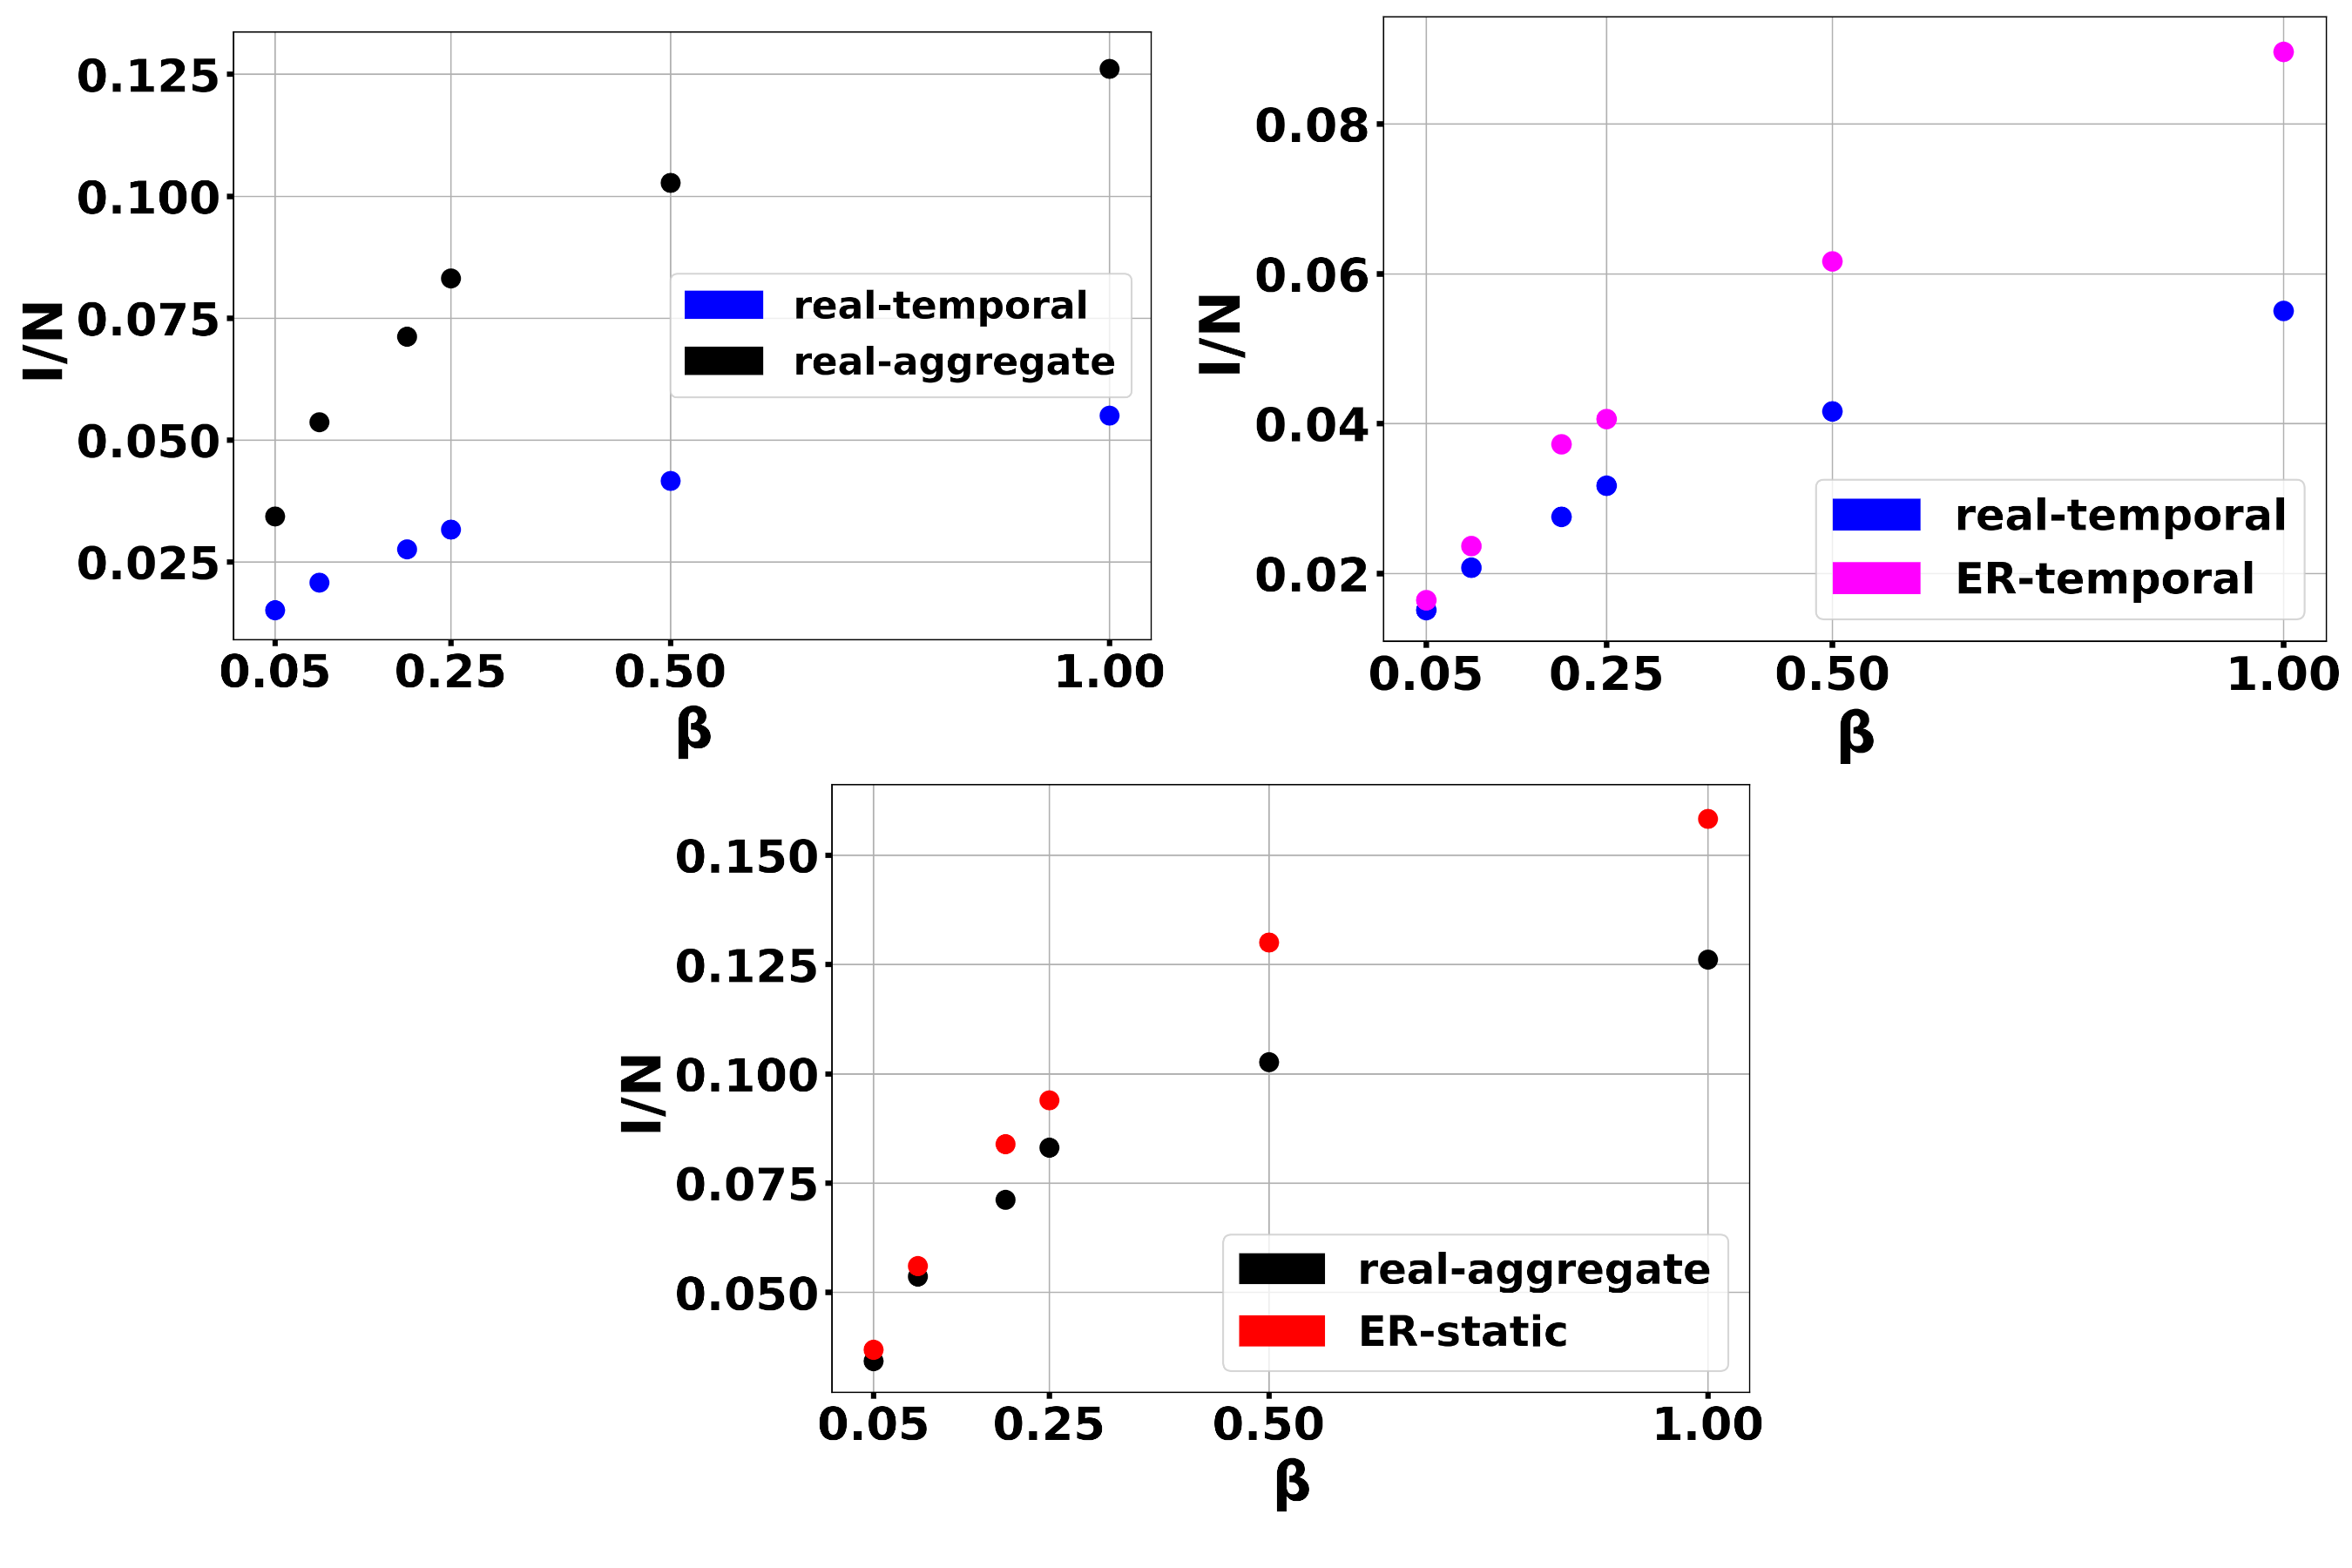
\includegraphics[width=\textwidth]{images/epidemics.png}
    \caption{Comparison of the final fraction $I/N$ of infected individuals. On the second day, the distribution of the degree and strength are wider compared to the other days: longer concats occured on the second day.}
    \label{fig:epidemics}
\end{figure}

On the top left of figure \ref{fig:epidemics}, \emph{real-aggregated} the fraction $g=I/N$ of infected individuals is greater than 2\% to 5\% with respect to \emph{real-temporal}: this is expected, as the strength (determining the transition from $S\rightarrow E$, see \eqref{eq:epidemic}) of the nodes in \emph{real-aggregated} are is significantly largerthan than the one of \emph{real-temporal}'s nodes. Similarly,  in the other figures the surrogate networks display larger values of $g$ than their temporal and aggregated counterparts. In all case, the difference increases with $\beta$.
Relaxing specific features of the dataset yields to uncompatible results and indicates that the real topology and interaction sequence of the event has a fundamental role in the spread of the epidemics.

\newpage